\documentclass[a4j,12pt,onecolumn,oneside,final]{jreport}

%\usepackage{gthesis}
\usepackage{gthesis_myown}


\usepackage{amsmath,amsthm,amssymb,ascmac}
\usepackage{fancybox}
\usepackage{slashbox}
%\usepackage[dviout]{color,graphics}
\usepackage[dvipdfmx]{graphicx}
\usepackage{color}
\usepackage{psfrag}
%\usepackage{upgreek}
\usepackage{bm}
\usepackage{wrapfig}
\usepackage{subcaption}

%%%%%%%%%%%%%%%%%%%%%%%%%%%%%%%%%%%%%%%%%%%%%%%%%%%%%%%%%%%%%%%%
% put local tex-macros in this file %

%%%%%%%%%%%%%%%%%%%%%%%%%%%%%
%色設定
%%%%%%%%%%%%%%%%%%%%%%%%%%%%%
\definecolor{Black}{rgb}{0.0,0.0,0.0}
\definecolor{Red}{rgb}{0.9,0.0,0.1}
\definecolor{Blue}{rgb}{0.1,0.1,0.5}
\definecolor{Green}{rgb}{0.1,0.4,0.1}
\definecolor{Gray}{rgb}{0.75,0.85,0.9} % Fuji-iro
\definecolor{Shade}{rgb}{0.1,0.1,0.4}

%%%%%%%%%%%%%%%%%%%%%%%%%%%%%%%%%%%%%%%%%%%%%%%%%%%%%%%%%%%%%%%%
\年度{令和1年度}
%\提出年月{平成30年7月}
\提出年月{令和1年1月}

\題名{構造特徴とattentionメカニズムを用いた \\GNNの半教師あり学習}
\梗概題名{構造特徴とattentionメカニズムを用いた\\GNNの半教師あり学習}
%\題名{楽に卒業する方法に関する基礎的研究\\
%			--- そもそもそれは可能か? ---}
%\梗概題名{楽に卒業する方法に関する基礎的研究\\
%			--- そもそもそれは可能か? ---}

\指導教員名A{村田 剛志}
\職名A{准教授}


%\所属学科{電気電子工学科}{}
\所属学科{情報工学科}{}
\学籍番号{16B16163}
\氏名{吉川 純平}

\内容梗概{近年、TwitterやFacebook等のSNS(ソーシャルネットワークサービス)の普及により、誰もがネットワーク上でのコミュニケーションが可能になったことや、化合物の物性推定の重要性の認識の高まりなどにより、グラフ構造を用いた解析が注目を集めている。グラフとはノードと、二つのノード間を結ぶエッジから構成されている。本研究ではグラフ構造とそれぞれのノードごとに備わっている構造特徴と少数のノードに備わったラベルにより、それ以外のノードのラベルを推定するための手法を提案する。

従来の研究ではグラフ構造において畳み込み演算をするグラフ畳み込みネットワークがラベル推定で高い精度を示している。しかしそのネットワーク1層では各ノードにおいて距離1で隣接したノードからの特徴をとることができず、ラベルの数が少ない場合は精度が低くなってしまう問題がある。そのため、グラフの構造特徴の学習も同時にさせる研究がなされるようになった。構造特徴とはグラフに構造からのみの情報により求められるものであり、主に中心性などが有名である。また、複数の入力のうちどの入力を重要視するかを決定するニューラルネットワークの手法であるattentionメカニズムを用いた手法が、近年グラフニューラルネットワークや画像認識などのさまざまな分野において高い精度を示すことが認識されてきた。

本研究では、グラフ畳み込みネットワークにおける学習に加えて、attentionメカニズムを用いてノードごとの中心性の重要度を測定し、それに比例した構造特徴の学習も両立させるようなモデルを実装した。この手法においては、近隣ノードの学習とグラフ全体の学習を可能にしている。

実験の結果、主にラベルが少ない場合に既存手法を上回る分類精度を得ることが確認できた。
}


\begin{document}
% ----------------------------------------------------------------------
% 表紙
\maketitle
% ----------------------------------------------------------------------
% 目次
\setcounter{page}{1}
\renewcommand{\thepage}{\roman{page}}
\setcounter{tocdepth}{1}
\tableofcontents
\clearpage
% ----------------------------------------------------------------------
% 内容
\setcounter{page}{1}
\renewcommand{\thepage}{\arabic{page}}
%\chapter{Introduction}
\chapter{序論}
\section{研究の背景と目的}
近年、TwitterやFacebook等のSNS(ソーシャルネットワークサービス)の普及により、誰もがネットワーク上でのコミュニケーションが可能になったことや、化合物の物性推定の重要性の認識の高まりなどにより、グラフ構造を用いた解析が注目を集めている。グラフとはノードと、二つのノード間を結ぶエッジから構成されている。グラフ構造を用いたデータ解析のタスクには、ノードの分類、ノードのクラスタリング、グラフ分類、リンク予測などがある。

本研究ではグラフ構造とそれぞれのノードごとに備わっている構造特徴と少数のノードに備わったラベルによる学習を用いて、ラベルの与えられていないノードにおけるノードのラベルを予測するようなタスクを行う。このタスクはラベルが分かっているノードとラベルが分かっていないノードのどちらにおいてのノードもグラフ構造と特徴量が分かっているため半教師あり学習という分野の研究である。このタスクはwebページ関係ネットワークのトピックを予測したり、SNS上でのユーザー関心の予測などがある。

このタスクにおいてはグラフベース正則化\cite{LP},\cite{chebnet},\cite{manireg},\cite{semiemb}が古くから研究されている。この手法は、ラベル付きノードに隣接しているノードはそのラベルと等しいラベルを持っているのではないかという推測に基づいた手法であるが、モデルが直感的であり表現力の向上が困難であった。それからグラフの構造をベクトル空間に埋め込むネットワークエンベディング\cite{embedding}の研究が盛んに行われている。この手法を用い、グラフから得たベクトル表現を機械学習モデルで学習させることで、ノード分類やリンク予測において高い精度を得ることが可能になった。この手法の欠点として、タスクによりどのようなベクトル表現を得るべきかを推論することが難しいことが上げられる。

近年、グラフにおいて畳み込み演算を行うグラフ畳み込みネットワークが高い精度を示している。グラフ畳み込み演算にはグラフフーリエ変換を用いる手法と、行列演算を用いて直接的に求める方法の2種類存在する。しかしそのネットワーク1層では各ノードにおいて距離1で隣接したノードからの特徴をとることができず、ラベルの数が少ない場合は精度が低くなってしまう問題がある。そのため、グラフの構造特徴の学習も同時にさせる研究がなされるようになった。構造特徴とはグラフに構造からのみの情報により求められるものであり、主に中心性などが有名である。また、複数の入力のうちどの入力を重要視するかを決定するニューラルネットワークの手法であるattentionメカニズムを用いた手法が、近年グラフニューラルネットワークや画像認識などのさまざまな分野において高い精度を示すことが認識されてきた。

本研究では、グラフ畳み込みネットワークにおける学習に加えて、attentionメカニズムを用いてノードごとの中心性の重要度を測定し、それに比例した構造特徴の学習も両立させるようなモデルを実装した。この手法においては、近隣ノードの学習とグラフ全体の学習を可能にしている。

実験の結果、主にラベルが少ない場合に既存手法を上回る分類精度を得ることが確認できた。

\section{本論文の構成}
本論文は全5章から構成される。第2章では本研究で利用する従来の手法や関連研究について述べる。第3章では本研究における提案手法について具体的に述べる。第4章では論文引用ネットワークを用いた実験を行う。第5章では本論文の結論と今後の課題について述べる。

%\chapter{Preliminaries}
\chapter{関連研究}

\section{グラフ構造}
\subsection{グラフ構造について}
グラフとはノードと、二つのノード間を結ぶエッジから構成されている。づまり、グラフをGとするとGは$G=(V,E)$として表せる。ここでV、Eはそれぞれノードの行列とエッジの行列である。エッジの種類にはエッジに向きがある有向グラフやあるノードから同じノードにエッジが張られるセルフループと呼ばれるエッジが存在するものや、同一ノード間に複数エッジが張られるものや、エッジに重みが備わっているものが存在するが、本研究では無向重みなしグラフを用いることにする。エッジのノード数をnとすると、隣接行列Aは$A \in R^{n\times n}$の行列を用いて、ノード$v_i$とノード$v_j$間にエッジがあるとき、Aのi行目j列目の要素$A_{ij}$が1となり、それ以外の場合で0とすることで表現できる。

\begin{figure*}[h]
  \centering
  \includegraphics[width=0.7\hsize]{figures/graph_structure.pdf}
  \caption{グラフ構造}
  \label{fig:ex1}
\end{figure*}

\subsection{グラフ構造を用いたタスクについて}
グラフを用いたタスクについては\cite{link-mining}によると以下のようなものがある。
\begin{itemize}
\item ノードごとのタスク
	\begin{itemize}
	\item ノードの分類
	\item ノードのクラスタリング
	\item ノードのランキング
    \item ノードの特定
	\end{itemize}
\item エッジごとのタスク
	\begin{itemize}
	\item リンク予測
	\end{itemize}
\item グラフ全体によるタスク
	\begin{itemize}
    \item 部分グラフの特定
    \item グラフ分類
    \item グラフ生成モデルの作成
	\end{itemize}
\end{itemize}

これらは近年、多くの研究がされている。また、本研究においてはノードごとのタスクである、ノード分類のみを研究対象にしている。

\section{半教師ありノード分類}
半教師ありノード分類問題は、グラフ全体の構造、それぞれのノードにおける特徴量、少数のラベルを用い、ラベルが与えられてない残りのノードのラベル予測をするタスクである。

グラフを$G=(V,E)$、$N = |V|$を用いて隣接行列をA$A \in R^{N\times N}$とする。特徴行列の集合を$X = \{x_{1},..., x_{n}\}$とする。用いるラベルの個数をlとし、ラベルのノードの集合を$V = \{ v_{1}, . . . , v_{l}, v_{l+1}, . . . , v_{N}\}$とする。それぞれのノードのラベルを$x_{1}, ..., x_{n}$とする。これらにより、半教師あり分類問題は以下のように定義される。


\begin{itemize}
\item 入力:\\
隣接行列:$A\in R^{N\times N}$,\\
全ノードの特徴ベクトル:$X=\{x_{1}, ..., x_{n}\}$,\\
$l$個の教師ラベル: $y_{1}, ...., y_{l}$
\item タスク:\\
ラベルなしノード$v_{l+1}, ..., v_{n}のラベル推定$
\end{itemize}

グラフを用いた半教師あり分類問題の重要な特徴の一つであることは、入力におけるノードのラベル数に関わらずに全てのノードにおけるグラフの構造と特徴行列を用いることができることである。
そのため、ラベル数が少ない半教師あり分類問題のようにラベルがとても少ない場合においては、グラフの構造とそれぞれのノードの特徴量をいかに利用するかが重要である。

\subsection{既存のアプローチ}
グラフを用いたノード分類の分野においては大きく分けるとグラフ正則化、グラフエンベディング、グラフニューラルネットワークの3つがある。本研究はグラフニューラルネットワークを用いた手法であるが、他の二つの手法についてこの章で簡単に述べる。
\subsubsection{グラフベース半教師あり学習}
グラフベース半教師あり学習66は古くから研究されている手法である\cite{manireg}。この手法の代表的なものがLabel Propagation\cite{LP}である。この手法はあるラベルのノードに隣接するノードはそのラベルである確率が高いであろうという経験的な推論に基づいた手法である。
\subsubsection{グラフエンベディング}
図\ref{fig:ex1}にように、グラフエンベディングはグラフ構造からベクトル空間に埋め込む手法のことである。それぞれのノードをベクトル空間に埋め込み、機械学習の手法を用いることでノード分類をすることを可能にしている。skip-gramモデル\cite{skip-gram}を用い、グラフにおけるランダムウォークをすることにより得られたノード列から分散表現を得たのがDeepwalk\cite{DeepWalk}と呼ばれる手法が最初に提案されて以降、それを応用した様々な研究がされている\cite{LINE}\cite{node2vec}。
エンベディングの手法はタスクによりどのようにベクトル空間に埋め込むべきかということを実際に考えなければならないため、良いモデルを作成することが難しいという欠点がある。



%ネットワークエンベディングは,ネットワーク構造からノードの低次元のベクトル表現を獲得する手法である.1つ1つのノードを特徴空間の点として表現することで,従来の機械学習アルゴリズムを適用することが可能になる.2014年にDeepWalk\cite{DeepWalk} が提案されて以来,数多くの研究が行われている.エンベディングで得られた分散表現を機械学習モデルの入力とすることで,既存の手法よりもラベル推定や分類タスクの精度を大きく向上させることに成功している.DeepWalkは,ランダムウォークによって得られたノードの系列に対し,skip-gramモデル\cite{skip-gram}を用いることで分散表現を得る手法である.その他にも,LINE\cite{LINE}やnode2vec\cite{node2vec}など,skip-gramをベースにした数多くの派生研究が行われている.
%エンベディングを用いて分類問題などのタスクを解く場合,分散表現を生成した後,機械学習モデルの学習を行うという二つのプロセスを行う必要がある.そのため,エンベディングによる手法では,特定のタスクに最適化した学習を行うことは難しいという欠点がある.また,パラメータの数はノード数に応じて線形的に増加するため,計算量が非常に大きいという問題もある.




\begin{figure*}[h]
  \centering
  \includegraphics[width=0.7\hsize]{figures/embedding.pdf}
  \caption{グラフエンベディングの可視化}
  \label{fig:ex1}
\end{figure*}







\section{グラフ畳み込みネットワーク}
\subsection{グラフニューラルネットワーク}
グラフニューラルネットワークは

\subsection{畳み込みニューラルネットワーク}
ディープラーニングが注目を浴びるようになった大きな要因として畳み込みニューラルネットワークを用いた手法\cite{imagenet}が画像認識の分野で高い精度を誇ったことがある。畳み込みニューラルネットワークのモデルは、画像の1辺のピクセル数に対してそれより1辺が小さいフィルタを移動させながら、画像のあらゆる畳み込み演算をするようなものである。このような作業を終えることで、行列変換をすることによりパラメータの数を減らし汎化性能を高めている。

\begin{figure*}[h]
  \centering
  \includegraphics[width=\hsize]{figures/cnn.pdf}
  \caption{畳み込みニューラルネットワーク中間層の構成}
  \label{fig:ex1}
\end{figure*}

しかし、画像認識の分野と違い、グラフ構造においては、各ノードごとがある規則により並んでいるわけではないため、畳み込み演算を用いることはできない。
グラフを用いた畳み込み演算アプローチにはグラフフーリエ変換を用いるspectral convolutionと直接的に行うspatial convolutionの2種類が存在する。

\subsection{spectral convolution}
グラフを用いて信号処理するアプローチ\cite{gsp}を用いてグラフ畳み込み演算を定義する方法がspectral convolution\cite{spectral}である。この手法は、グラフラプラシアンの固有値分解により、グラフ上のデータをグラフ信号として扱い、信号の急峻さで成分分解し、要素積を求め、それを逆フーリエ変換するという手法である。

また、この手法は計算コストが大きいため,\cite{chebnet}では計算量を減らすためにチェビシェフ近似を用いている。

\vspace{1cm}

\begin{figure*}[h]
  \centering
  \includegraphics[width=0.5\hsize]{figures/filtering.eps}
  \caption{spectral convolution\cite{spectral}}
  \label{fig:ex1}
\end{figure*}


\subsection{spatial convolution}
spectral convolutionは数学的に有力な手法であると証明されているが、この手法の問題点として、計算量が大きいことや、セルフループや多重辺を持つ場合に適応させられないという問題がある。そこで、グラフ構造のエッジの構造に着目し、畳み込み演算を用いる手法が提案された\cite{message}。その操作1回における畳み込み演算は、ノードiにおいてそのノード自身と、そのノードにエッジを張るノードからのみによって、特徴行列が更新されていくというものである。ノードiにおける1回の畳み込み演算の式は以下の通りである。
$$ \displaystyle h^{(l+1)}_i = \sigma \left(h^{(l)}_i W^{(l)}_0 + \sum_{j \in \mathcal{N_i}} \frac{1}{c_{i, j}} h^{(l)}_j W^{(l)}_1  \right). $$
$c_{i,j}$は正規化のための定数であり、$c_{i,j} = |N_i|$である。$N_i$はノードiにエッジを張るノードの集合である。


\begin{figure*}[h]
  \centering
  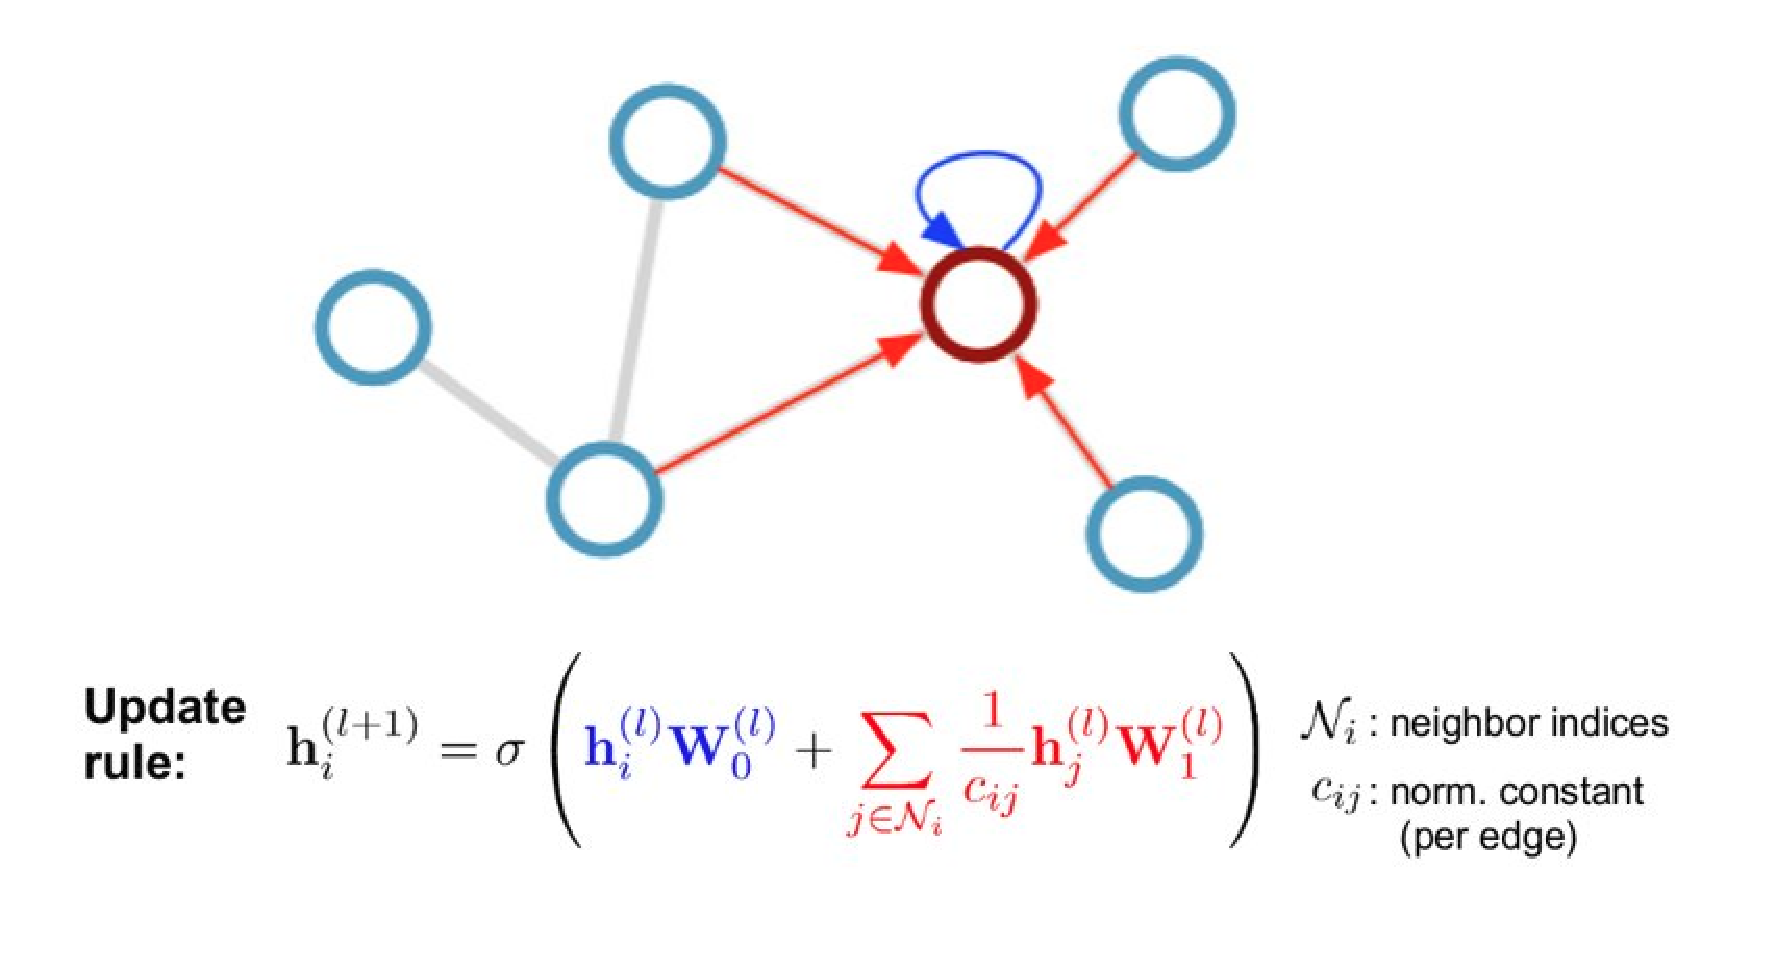
\includegraphics[width=0.7\hsize]{figures/spatial.eps}
  \caption{spatial convolution\cite{gcn}}
  \label{fig:ex1}
\end{figure*}

\section{グラフ畳み込みネットワーク}
$g_{\theta}$をチェビシェフ多項式として近似することにより、spactral convolution を spatial convolutionに近似できるという手法がグラフ畳み込みネットワーク\cite{gcn}である。
グラフ畳み込みネットワークの第$i$層の出力は以下の式で表せる。
\begin{equation}
H^{(i)} = \sigma(D^{-1/2}\tilde{A}D^{-1/2}H^{(i-1)}W^{(i)})
\end{equation}

ここで、$\tilde{A}=A+I_{n}$,$I_{n}\in \mathcal{R}^{n \times n}$は単位行列、$D \in \mathcal{R}^{n \times n}$は次数行列、$H^{(0)}=X$、$W^{(i)}$は$i$層における特徴行列を更新するための重み行列である。また、$\sigma$はReLU関数やsigmoid関数などの活性化関数である。また、教師あり目的関数のロス関数は下の式で更新される。

\begin{equation}
L_{supervised} = - \sum_{l \in y_{l}} \sum_{f=1}^{F} Y_{lf} lnZ_{lf}
\end{equation}
ここで、$y_{l}$はラベル与えられているノード、$Y$はラベル行列、$Z$はグラフ畳み込みネットワーク全体を通しsoftmax関数によって計算される行列である。
この手法はエンドツーエンド学習されている。

\begin{figure*}[h]
  \centering
  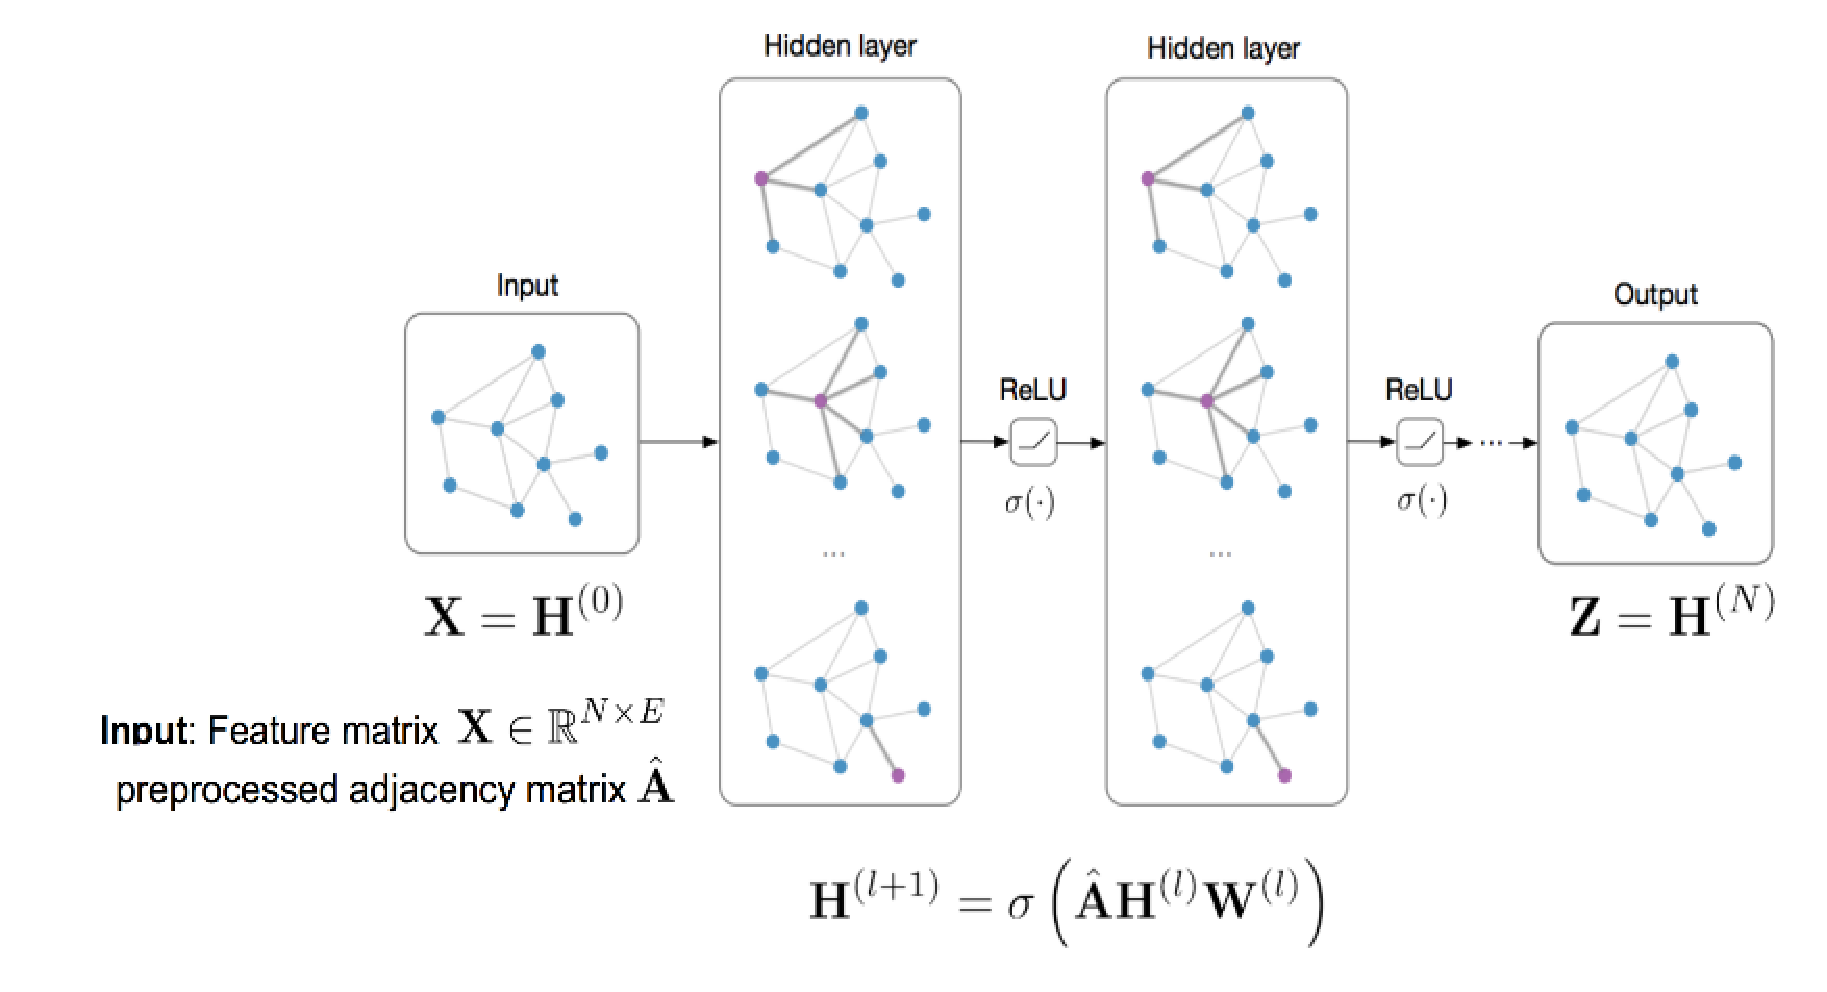
\includegraphics[width=1.0\hsize]{figures/gcn.eps}
  \caption{グラフ畳み込みネットワーク\cite{gcn}}
  \label{fig:ex1}
\end{figure*}





\section{構造特徴}
複雑ネットワークにおいて、そのグラフの特徴を図るための特徴量として構造特徴がある。構造特徴にはグラフ全体を数値で表すグラフ全体構造特徴と、グラフのノードごとを数値で表すノードごとの構造特徴が存在する。
\subsection{グラフ全体の構造特徴}
任意の頂点間の距離の平均を表す平均距離や、グラフ全体におけるエッジによりできたクラスタ(三角形)の個数により定まるクラスター係数などがある。また、これらはグラフ全体において1つの値しか持たないため、ノード分類においてこの特徴量を利用することは難しい。

\subsection{ノードごとの構造特徴}
これらは、グラフにおいて、ノードごとに一つの値が決定されるため、ノード分類の分野に適応しやすい特徴量である。
\begin{itemize}
\item 媒介中心性\\
ノードiが任意のノードペアの最短経路にどれだけ含まれているかを表す指標である。
$$C_i = \frac{\sum_{j<k} path_{jk}(i)/path_{jk}}{(N-1)(N-2)} $$
$path_{jk}$はノードj, k間の最短経路の総数,$path_{jk}(i)$は
その中でノード $i$ を経路に含む最短パスの総数である。
\item 近接中心性\\
ノード$v_{i}$の近接中心性は,ノード$v_{i}$から他のノードまでの平均距離によって定義される。平均的に他のノードに近いほど値は大きくなる。
$$C_i = \frac{N-1}{\sum_j d(v_i,v_j)} $$

\item 次数中心性\\
グラフにおいての他のノードとどの程度直接つながっているのかを表す指標である。$k_{i}$をノード$i$に直接張られたエッジの総数であるとすると ノード$i $の中心性$C_{i}$は以下である。
$$C_i = \frac{k_{i}}{N-1} $$

\item 固有ベクトル中心性\\
ノード$v_{i}$の固有ベクトル中心性は、ノード$v_{i}$と隣接したノードがどれだけ中心性をもっているかという指標である。
$$C_i = \sum_{j} A_{ij} C_j $$
$A_{ij}$は隣接行列の要素である。ノードiからノードjにエッジが張られていたら1,そうでなければ0である。この式の繊維を繰り返し最終的に収束する値$C_i$が求める中心性となる。

\item PageRank\cite{pagerank} \\
pagerankはweb検索に用いられる手法であり、評価の高いページからリンクが多く張られるほどよいページであるというアルゴリズムを用いた手法である。
$$ PR(A) = (1-d) + d \sum_{i=1}^{n} \frac{PR(T_{i})}{C(T_{i})}$$
ここで、$PR(T_{i})$はノード $i$に直接エッジを張っているノードの重要度,$C(T_{i})$はノード$i$に張られたエッジの総数である。dはトレードオフパラメータである。
\end{itemize}
% 上記の他にも,HITS,Katz中心性,フロー中心性,ボナチッチ中心性など,数多くの指標が存在する.

\section{attentionメカニズム}
近年、attentionメカニズムというモデルを使った手法\cite{bahdanau2014neural}\cite{attention}が機械翻訳の分野において高い精度を出し注目を浴びている。attentionメカニズムの一つのやり方として、ベクトル内積を用いて二つのものの類似度をとることにより、必要な情報により多くの注意を払うものである。
例えば下図のように、attentionメカニズムとは自然言語処理の分野において、'making'というqueryが与えられた時に'more'や'difficult'というkey-valueがそのqueryが注意の重みを大きくしていることが分かる。

\begin{figure*}[h]
  \centering
  \includegraphics[width=0.5\hsize]{figures/attention_mechanism.pdf}
  \caption{attentionを用いたモデル\cite{attention}}
  \label{fig:ex1}
\end{figure*}

\begin{figure*}[h]
  \centering
  \includegraphics[width=1.0\hsize]{figures/attention_visualization.pdf}
  \caption{attentionを用いた単語間関係の可視化\cite{attention}}
  \label{fig:ex1}
\end{figure*}
\newpage{}

\chapter{先行研究}
\section{構造特徴を用いたグラフ畳み込みネットワーク}
グラフ畳み込みネットワーク\cite{gcn}をベースにし、グラフの構造特徴の情報も学習させたモデルが提案された\cite{GCN_SS}。手法の概形は図\ref{fig:architecture}の通りである。

\begin{figure*}[htbp]
  \centering
  \includegraphics[width=1.0\hsize]{figures/simple.eps}
  \caption{\cite{GCN_SS}の手法(2層グラフ畳み込みネットワークを用いたモデル)}
  \label{fig:architecture}
\end{figure*}

\newpage{}


\begin{figure*}[htbp]
  \centering
  \includegraphics[width=1.0\hsize]{figures/GCN_SS.pdf}
  \caption{\cite{GCN_SS}の手法のおよその流れ}
  \label{fig:architecture}
\end{figure*}


この手法においては、グラフ畳み込みネットワークの目的関数に構造特徴を保持する項を加えることにより、教師あり学習の目的関数と教師なし学習の目的関数のどちらも最適化しようとする手法である。教師あり損失関数は、グラフ畳み込みネットワークと同じ構造を用いラベル予測をするものであり、教師なし損失関数では、畳み込みネットワーク1層目における出力において構造特徴を保持するに学習するモデルとなっている。構造特徴の目的関数はトレードオフパラメータ$\alpha$を用いて表される。
\begin{equation}
L = (1-\alpha) L_{supervised} + \alpha L_{unsupervised}
\end{equation}
ここで、$L_{supervised}$は教師あり学習によって求まる損失関数であり、$L_{unsupervised}$は教師なし学習によって求まる損失関数である。

\subsection{教師あり損失関数}
教師あり学習におけるラベル予測は\cite{gcn}で用いられるものと同じであり、教師あり損失関数は以下のようになる
\begin{equation}
L_{supervised} = - \sum_{l \in Y_{l}} \sum_{f=1}^{F} Y_{lf} lnZ_{lf}
\end{equation}
ここで$Y_{l}$はラベル付けされたノードの場合1、それ以外で0で表される。

\subsection{構造特徴行列の計算}
構造特徴は、入力行列である隣接行列により、各ノードごとの構造特徴をそれぞれ計算される。提案手法で用いる構造特徴はノードごとに計算される中心性である、媒介中心性、近接中心性、次数中心性、固有ベクトル中心性、pagerankなどである。それぞれのノードごとの特徴量を全ての構造特徴において結合したものを構造特徴行列$ R\in R^{N\times S}$とする。Nはノード数、Sは用いる構造特徴の総数である。この構造特徴は使うデータセット によって一意に定まるため、一度計算したら再度計算する必要性はないため、モデル全体の計算量に対する影響はとても低い。

\subsection{教師なし損失関数}

提案手法においては、2層のグラフ畳み込みネットワークを用いる。1層目の畳込み層の関数を$GCN_1$、2層目の畳込み層の関数を$GCN_2$とすると、グラフ畳み込みネットワークにおける順伝播は以下の式で表せる。\\
\begin{eqnarray}
H_{hid} = GCN_1(X,A)\\
H_{out}=GCN_2(H_{hid} , A)
\end{eqnarray}
構造特徴保持のための学習を$H_{hid}$からそれぞれのノードにおける特徴ベクトル$\hat{R}$を計算する層を導入する。2層のグラフ畳み込みネットワークを用いる場合は、1層目の畳み込み層における出力から派生させて特徴ベクトルを計算する。それぞれのノードにおける重みパラメータ{\bf $\omega$}を用いることで特徴ベクトル$\hat{R} \in R^{N\times S}$は以下のように計算できる。
\begin{equation}
\hat{R} = f(w, H_{hid})
\end{equation}

出力された特徴ベクトルが,グラフ構造から計算された構造特徴と等しくなるように学習を行うことで,構造特徴の保持を行う.グラフから計算した構造特徴と出力された特徴ベクトルの2乗誤差を用いて損失関数の計算を行う.
\begin{equation}
L_{unsupervised} = \sum_{i=1}^{N} ||R_{i} - \hat{R_{i}}||^{2}
\end{equation}





%\chapter{Main Results}
\chapter{提案手法}


本研究では「2層の畳み込みニューラルネットワークに構造特徴を追加したモデル」にattentionメカニズムを適応したモデルを提案する。モデルの概要は以下の通りである。
\begin{figure}[htbp]
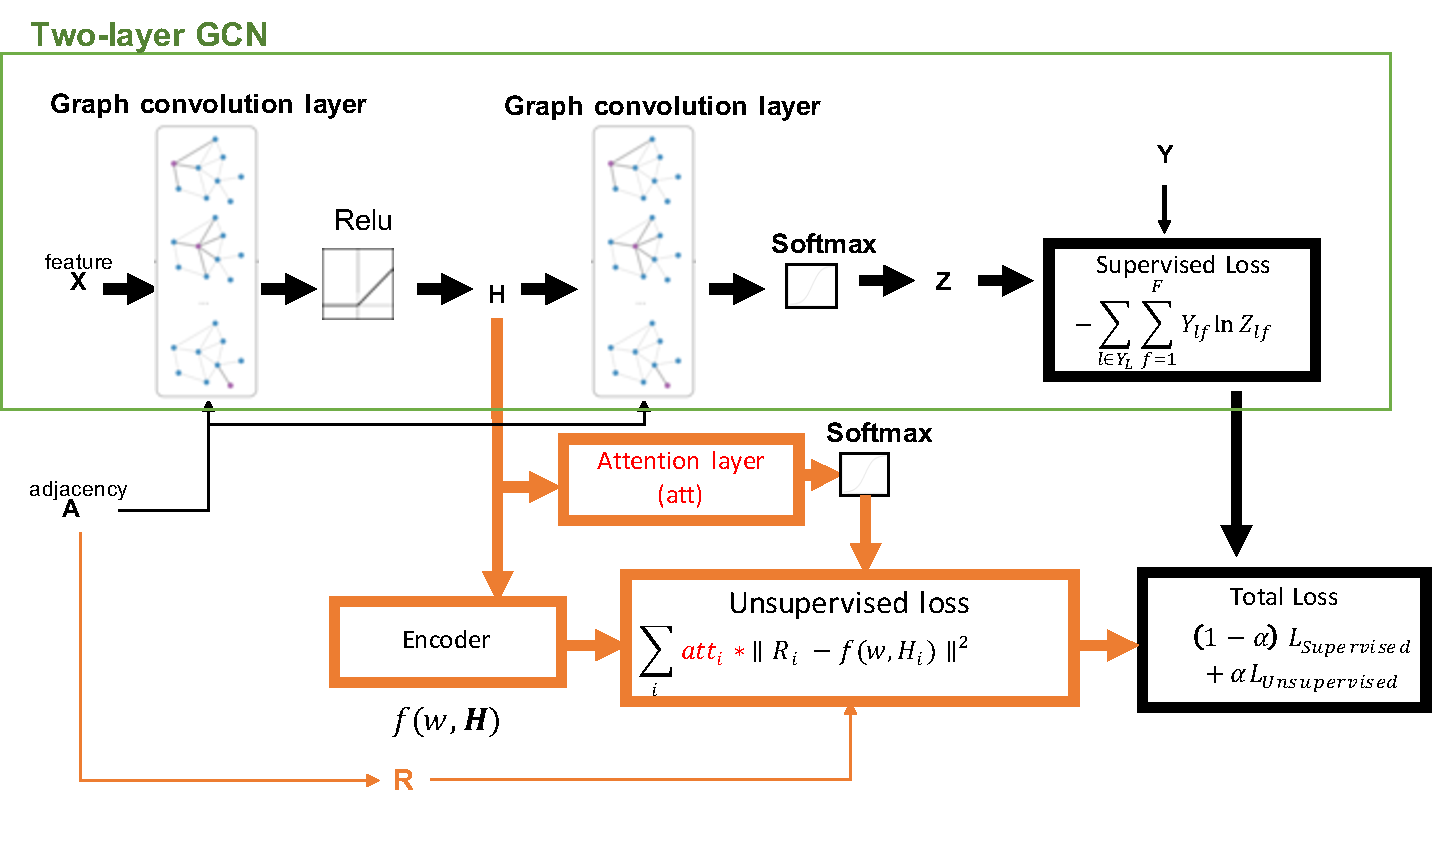
\includegraphics[width=1.0\hsize]{figures/proposed2.pdf}
\caption{提案手法(2層GCNを用いたモデル)}
\label{fig:architecture}
\end{figure}
\\
\\
\section{提案手法}
提案手法の図は図3.1に示す。図の上側にある緑枠で囲まれた部分はGCNの元論文の実装と等しい畳み込みネットワークである。図の下側にあるネットワークは構造特徴を用いて損失関数を出力する層になっている。提案手法においては本来のGCNで求める教師あり学習と構造特徴にattentionメカニズムを組み込んで求める教師なし学習、これら二つの目的関数を最適化するような目的関数を求めるものである。具体的にはトレードオフパラメータ$\alpha $を用い以下のような目的関数を実装することにより実現している。
\begin{equation}
L = (1-\alpha) L_{supervised} + \alpha L_{unsupervised}
\end{equation}
ここで、$L_{supervised}$は教師あり学習の損失関数、$L_{unsupervised}$は教師なし学習の損失関数である。
教師あり学習の損失関数は教師データのラベルのみを使い学習され、教師なし学習の損失関数は全てのノードにおいて学習される。また、およその流れは以下の図のようになっている。
\begin{figure}[htbp]
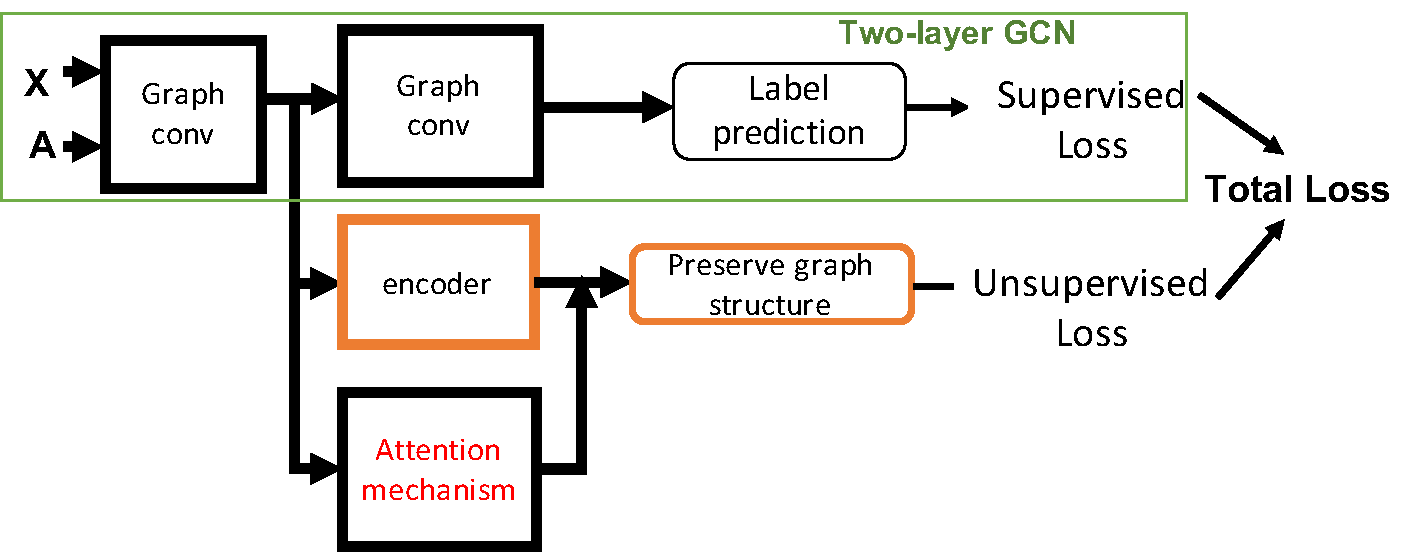
\includegraphics[width=1.0\hsize]{figures/proposed.pdf}
\caption{提案手法のおよその流れ}
\label{fig:flow}
\end{figure}
\section{教師あり学習における損失関数}
教師あり学習においては,\cite{gcn}でのラベル予測学習で用いられる損失関数と同様の損失関数を用いる。入力には隣接行列Aと特徴行列Xを使用し、ニューラルネットワークにおける順伝搬によって演算が行われる。ここで、特徴行列Xは、それぞれのノードが個別に持っているそのノードの特徴を表す行列である。ネットワーク$i$層における出力は以下のようになる。
\begin{equation}
Z^{(i)} = \sigma(D^{-1/2}\tilde{A}D^{-1/2}Z^{(i-1)}W^{(i)})
\end{equation}
ここで,$\tilde{A}=A+I_{n}$,$I_{n}\in R^{n \times n}$は単位行列であり、$\tilde{D_{i,j}}$は、
\begin{equation}
\tilde{D_{i,j}} = \begin{cases}
    \sum_j \tilde{A_{i,j}} & (i==j) \\
    0 & (otherwise)
  \end{cases}
\end{equation}
である。\\

ネットワークの入力ベクトル$Z^{(0)}$を特徴ベクトルX,$W^{(i)}$をネットワーク中の$i$層における重み行列であり,$\sigma(.)$はReLU関数やシグモイド関数などの活性化関数とすると、畳み込み層が2層のニューラルネットワークを用いて,活性化関数を1層目にRelu、2層目にsoftmax関数を用いたとすると、出力は以下のように表される。
\begin{equation}
Z = f(X, A) = {\rm softmax}(\hat{A}{\rm ReLU}(\hat{A} XW^{(0)})W^{(1)})
\end{equation}





ここで、$ \hat{A} = \tilde{D}^{-1/2} \tilde{A} \tilde{D}^{-1/2} $と置く。$W^{(0)} \in \mathcal{R}^{C\times H}$は入力層から隠れ層へ変換するための重み行列であり、$W^{(1)} \in \mathcal{R}^{H\times F}$は,隠れ層から出力層へ変換するための重み行列である。変数C,H,Fはそれぞれ入力層、隠れ層、出力層のサイズを表すパラメータであり、Cは特徴量の次元数、Hはハイパーパラメータ、Fはノードのラベルの種類数によって定まる。損失関数は、ラベル付きノードにおいてのクロスエントロピーにより求められる。教師あり学習における損失関数は以下のようになる。
\begin{equation}
L_{supervised} = - \sum_{l \in Y_{l}} \sum_{f=1}^{F} Y_{lf} lnZ_{lf}
\end{equation}
ここで$Y_{l}$はラベル付けされたノードの場合1、それ以外で0で表される。


\section{教師なし学習における損失関数}
まず、構造特徴を保持するための学習についての詳細を説明する.

\subsection{構造特徴行列の計算}
構造特徴は、入力行列である隣接行列により、各ノードごとの構造特徴をそれぞれ計算される。提案手法で用いる構造特徴はノードごとに計算される中心性である、媒介中心性、近接中心性、次数中心性、固有ベクトル中心性、pagerankなどである。それぞれのノードごとの特徴量を全ての構造特徴において結合したものを構造特徴行列$ R\in R^{N\times S}$とする。Nはノード数、Sは用いる構造特徴の総数である。この構造特徴は使うデータセット によって一意に定まるため、一度計算したら再度計算する必要性はないため、モデル全体の計算量に対する影響はとても低い。

\subsection{特徴ベクトルの計算}

提案手法においては、2層のグラフ畳み込みネットワークを用いる。1層目の畳込み層の関数を$GCN_1$、2層目の畳込み層の関数を$GCN_2$とすると、グラフ畳み込みネットワークにおける順伝播は以下の式で表せる。\\
\begin{eqnarray}
H_{hid} = GCN_1(X,A)\\
H_{out}=GCN_2(H_{hid} , A)
\end{eqnarray}
構造特徴保持のための学習を$H_{hid}$からそれぞれのノードにおける特徴ベクトル$\hat{R}$を計算する層を導入する。2層のグラフ畳み込みネットワークを用いる場合は、1層目の畳み込み層における出力から派生させて特徴ベクトルを計算する。それぞれのノードにおける重みパラメータ{\bf $\omega$}を用いることで特徴ベクトル$\hat{R} \in R^{N\times S}$は以下のように計算できる。
\begin{equation}
\hat{R} = f(w, H_{hid})
\end{equation}

\subsection{attentionの計算}
構造特徴の保持を行うために、出力された特徴ベクトルがグラフそのものから計算された構造特徴との差異ができるだけ小さくなるように学習を行う。ここで、ノードごとに構造特徴の中で重要な構造特徴とそうでない構造特徴があるものに注目し、ノードごとに構造特徴にattentionメカニズムを組み込む。求める教師なし損失関数は、グラフから計算した構造特徴とグラフ畳み込みネットワークの1層から出力された特徴ベクトルの二乗誤差にノードごとの構造特徴においてattentionをかけたものとなる。
\begin{equation}
L_{unsupervised} = \sum_{i=1}^{N} att_i * ||R_{i} - \hat{R_{i}}||^{2}
\end{equation}
ここで、$att_i \in R^{S}$はノードiにおけるそれぞれの構造特徴にかかるattentionである。

%\chapter{Main Results}
\chapter{実験}

\section{モデル構成とパラメータ設定}
ネットワークにおける半教師あり学習におけるノードの分類問題のタスクにおいて実験を行った。モデルは2層のグラフ畳み込みネットワークを用い、隠れ層の活性化関数にはReLU関数、出力層の活性化関数にはソフトマックス関数を用いた。また、attention層の活性化関数にはソフトマックス関数を用いた。また、\cite{dropout}と重み減衰を用いて正則化を行った.グラフ畳み込みネットワークとattention層における重み行列は、Glorotの一様分布\cite{glorot}を用いて初期化した。最適化に用いる勾配降下法にはAdam\cite{Adam}を用いた。トレードオフパラメータ$\alpha$を用い、ラベル推測学習と構造特徴保持学習の損失を等しい割合で足し合わせたものを、最終的な目的関数として用いる.全ての実験はPython3.7で動作しており、ニューラルネットワークにおけるモデルや最適化のライブラリとしてpytorchを用いた。構造特徴の計算には、NetworkXを用いた。\\
 比較手法と平等に比較するために、ハイパーパラメータは\cite{gcn}における実験と同様の値を用いる。
 最大エポック数は200、学習率は0.01、ドロップアウト率は0.5隠れ層のサイズは32とする。また、validationセットにおける損失関数が10エポック間において減少しない場合は学習を打ち止めにするようにする。また、構造特徴は媒介中心性、近接中心性、次数中心性、固有ベクトル中心性、pagerankの5つ全てを用い実験する。
\begin{table}[h]
\begin{center}
\label{parameter}
\caption{パラメータ設定}
  \begin{tabular}{l|c} \hline
  パラメータ & 値 \\ \hline
  学習率 & 0.01 \\
  エポック数 & 200 \\
  隠れ層のユニット数 & 32 \\
  ドロップアウト率 & 0.5 \\
  重み減衰パラメータ & 5e-4\\ \hline
  %トレードオフパラメータ$\alpha$ & 0.5 \\   \hline
  \end{tabular}
  \end{center}
\end{table}

\section{データセット}
本実験で使用するデータセットはcora、citeseer、pubmedの3つであり、これらはどれも論文間の引用関係に基づいたネットワークである。これらのネットワークはノードを論文、エッジを論文の引用関係、ラベルをその論文がどの分野の論文であるかを表す。特徴ベクトルはそれぞれの論文の概要からbag of wordsを用いて、その概要に含まれる単語を抽出し表されている。データセットの概要と可視化を表\ref{dataset}と図\ref{fig:dataset}により示す.

論文の引用関係ネットワークにおいては,ノードは論文,エッジは論文の引用関係,ラベルはその論文が属する分野を表す.また,論文の概要をBag of Wordsを用いて抽出したものを特徴ベクトルとして用いている.それぞれのデータセットを可視化したものを図\ref{fig:dataset}に示す.



\begin{table}[h]
\begin{center}
\caption{データセット}
\label{dataset}
  \begin{tabular}{l|crrrrr} \hline
    &  ノード & エッジ & クラス & 特徴量  \\ \hline
    Cora & 2,708 & 5,429 & 7 & 1,433 \\
    Citeseer  & 3,327 & 4,732 & 6 & 3,703 \\
    Pubmed  & 19,717 & 44,338 & 3 & 500 \\ \hline
  \end{tabular}
  \end{center}
\end{table}

\begin{figure}%[H]
  \begin{center}
    \begin{tabular}{c}
    
    \begin{minipage}{0.5\hsize}
  \centering
  \includegraphics[width=6cm]{figures/cora.eps}
  \subcaption{Cora}
  \label{cora_vis}
\end{minipage}\\

\begin{minipage}{0.5\hsize}
  \centering
    \includegraphics[width=6cm]{figures/citeseer.eps} 
    \subcaption{Citeseer} %タイトルをつける
    \label{citeseer_vis} %ラベルをつけ図の参照を可能にする
\end{minipage}

\begin{minipage}{0.5\hsize}
  \centering
    \includegraphics[width=6cm]{figures/pubmed.eps} 
    \subcaption{Pubmed} %タイトルをつける
    \label{pubmed_vis} %ラベルをつけ図の参照を可能にする
\end{minipage}
    \end{tabular}
    \caption{各データセットの可視化}
    \label{fig:dataset}
  \end{center}
\end{figure}

\clearpage

\section{比較手法}
比較手法には、グラフ上で教師ありラベルの備わったノードから他のノードにラベルを伝搬させる手法であるラベル伝搬法(LP)\cite{LP}、ランダムウォークにより、グラフをベクトル空間に埋め込む手法であるDeepwalk\cite{DeepWalk}、サンプリングによりラベル情報とグラフを用いエンべディングを行うPlanetoid\cite{planetoid}、本研究の教師あり学習のベースとなるGCN\cite{gcn}、そのGCNに構造特徴を組み込んだ手法(GCN+ss)\cite{GCN+ss}を用いた。
ここで、GCNとGCN+ss以外の手法においては実験を行わず、\cite{gcn}で示される結果を引用する。


\section{実験結果}
\subsection{ノードの分類精度}
\ref{weakness}で述べたように、教師ありノードの割合が少ない場合は、グラフ畳みん込みネットワークにおいて、精度が大きく落ちてしまう。それにより、各データセットにおいて用いる教師データの数を各クラス数に応じて変化させることにより分類精度を比較する。教師ありノードの割合は全体のノード数に対して、Cora、Citeseerにおいては1\%,2\%,3\%,4\%,5\%、pubmedにおいては0.1\%,0.2\%,0.3\%,0.4\%,0.5\%と変化させることにより精度をそれぞれの精度を比較した。各クラスごとに等しい数の教師ありラベルを用いた。クラスごとのラベル選択により偏りがでるため、300回の実験による平均した値を分類精度とした。また、バリデーションデータとして500個、テストデータとして1000個のラベル付きデータセットを用いて評価を行った。

各データセットにおけるノード分類の精度を表\ref{cora_result} - \ref{pubmed_result}に示す。GCNを使っていない手法においては論文から引用した数値を使っているため、表の一部が空欄になっている。

\begin{table}[h]
  \begin{center}
  \caption{学習時の教師ラベル数を変化させたときの分類精度}
    \begin{tabular}{c}

      % 1
      \begin{minipage}{0.7\hsize}
        \begin{center}
     \subcaption{Coraデータセットにおける分類精度}
	\label{cora_result}
        \begin{tabular}{l|ccccc} \hline
    教師ラベル数 &  1\% & 2\% & 3\% & 4\% & 5\%  \\ \hline
    LP & -- & -- & -- & -- & 68.0 \\
    DeepWalk & -- & -- & -- & -- & 67.2 \\
    Planetoid & -- & -- & -- & -- & 75.1 \\ \hline \hline
    GCN & 67.1 & 75.0 & 77.6 & 79.5 & 80.5 \\
    GCN+SS & 68.0 & 75.4 & 78.3 & 79.8 & 80.8 \\
    {\bf Proposed} & 68.8 & 75.8 & 78.0 & 79.8 & 80.8 \\ \hline
  \end{tabular}
        \end{center}
             \vspace{1cm}
      \end{minipage}\\
      
 
      
      % 2
      \begin{minipage}{0.7\hsize}
        \begin{center}
    \subcaption{Citeseerデータセットにおける分類精度}
\label{citeseer_result}
  \begin{tabular}{l|ccccc} \hline
    教師ラベル数 &  1\% & 2\% & 3\% & 4\% & 5\%  \\ \hline
     LP & -- & -- & -- & -- & 45.3 \\
    DeepWalk & -- & -- & -- & -- & 43.2 \\
    Planetoid & -- & -- & -- & -- & 64.7 \\ \hline \hline
    GCN & 60.4 & 66.3 & 68.3 & 69.5 & 70.2 \\
    GCN+SS & 62.0 & 67.3 & 68.8 & 69.9 & 70.5 \\
    {\bf Proposed} & 62.1 & 66.8 & 68.8 & 69.7 & 70.5 \\ \hline
  \end{tabular}
        \end{center}
          \vspace{1cm}
      \end{minipage}\\
      
    
      
          \begin{minipage}{0.7\hsize}
        \begin{center}
    \subcaption{Pubmedデータセットにおける分類精度}
\label{pubmed_result}
  \begin{tabular}{l|ccccc} \hline
    教師ラベル数 &  0.1\% & 0.2\% & 0.3\% & 0.4\% & 0.5\%  \\ \hline
     LP & -- & -- & -- & -- & 63.0 \\
    DeepWalk & -- & -- & -- & -- & 65.3 \\
    Planetoid & -- & -- & -- & -- & 77.2 \\ \hline \hline
    GCN & 71.0 & 75.5 & 77.5 & 78.8 & 79.8 \\
    GCN+SS & 71.8 & 75.4 & 77.3 & 78.2 & - \\
    {\bf Proposed} & 71.4 & 75.1 & 77.1 & 78.6 & 79.5 \\ \hline
  \end{tabular}
        \end{center}
      \end{minipage}

    \end{tabular}
  \end{center}
\end{table}



それぞれのデータセットにおける分類精度を評価したものを表\ref{cora_result} - \ref{pubmed_result}に示す.教師ラベル数とは,全てのノードのうちラベル付けされているノードの割合を表す.GCN以外の比較手法については,論文から引用した数値を用いたため,空欄となっている箇所がある.また,GCNと提案手法の精度を比較したグラフを図\ref{fig:cora_result} - \ref{fig:pubmed_result}に示す.横軸は学習データサイズ,縦軸は分類精度を表す.
全てのデータセットにおいて,提案手法が最も高い精度を示している.とくに,教師ラベルの数が少ない場合において,提案手法は既存手法よりも大きく精度が向上している.これは,教師ラベルが少ない場合には,構造特徴を用いることで,学習時の情報の少なさを補っているためだと考えられる.









\subsection{トレードオフパラメータの$\alpha$による推移}
提案手法においてはトレードオフパラメータ$\alpha$を用いて、教師ありの損失と教師なしの損失の重み付けをしている。このパラメータによりどれほど影響がでるかを調べるために実験を行った。attentionメカニズムを用いずに構造特徴を均等に教師なし学習させたモデルであるGCN\_ssと構造特徴にattentionメカニズムを組み込んだ提案手法を比較した。実験はハイパーパラメータ$\alpha$を0から1まで0.1刻みで値を変化させ、それぞれのデータセットにおいてそれぞれの$\alpha$で300回の施行を行い、精度の比較を行った。教師データの数はcora,citeseer,pubmedで各ラベルの種類ごとに4,7,6個(全体における1\%、1\%、0.1\%)用い、結果は図\ref{cora_alpha}、図\ref{citeseer_alpha}、図\ref{pubmed_alpha}のようになった。横軸はハイパーパラメータ$\alpha$、縦軸はノードの分類精度を表している。図から分かるように、$\alpha$=1に近い場合、分類精度が大きく低下しているが、これは構造特徴を用いた精度教師なし学習による学習の比率がほとんどを占めるため精度落ちていると推測できる。coraやciteseerにおいては$\alpha$=0の場合は構造特徴による学習がされていなく、精度が落ちていると考えられる。

\begin{figure*}[h]
  \centering
    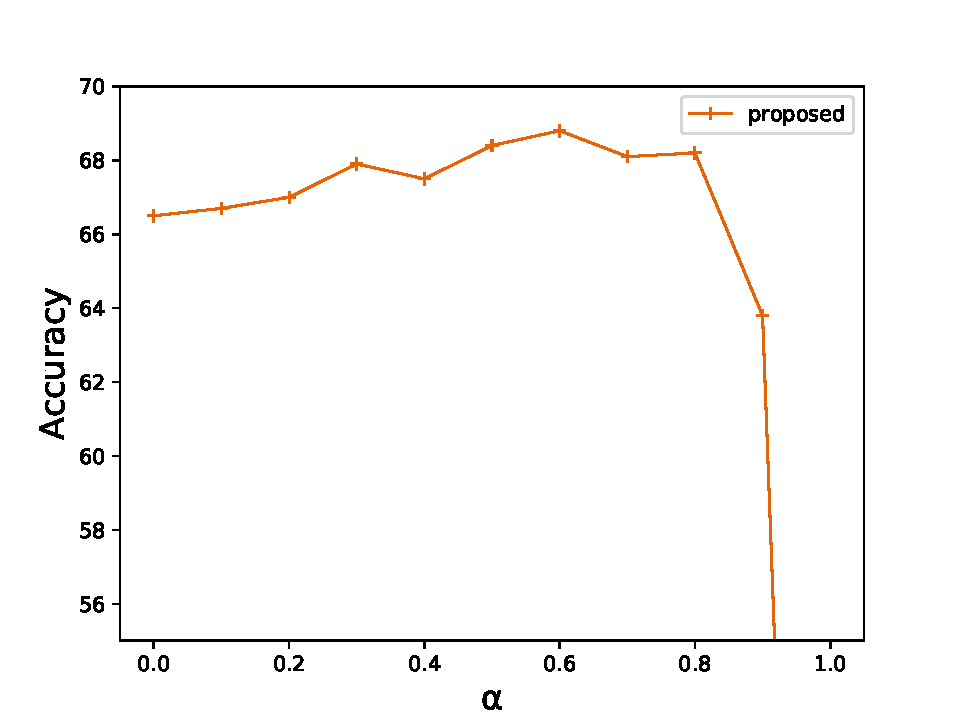
\includegraphics[width=12cm]{figures/cora_solo.pdf}
     \vspace*{0.5cm} 
    \caption{coraにおける比較} %タイトルをつける
    \label{cora_alpha} %ラベルをつけ図の参照を可能にする
\end{figure*}

\begin{figure*}[h]
  \centering
    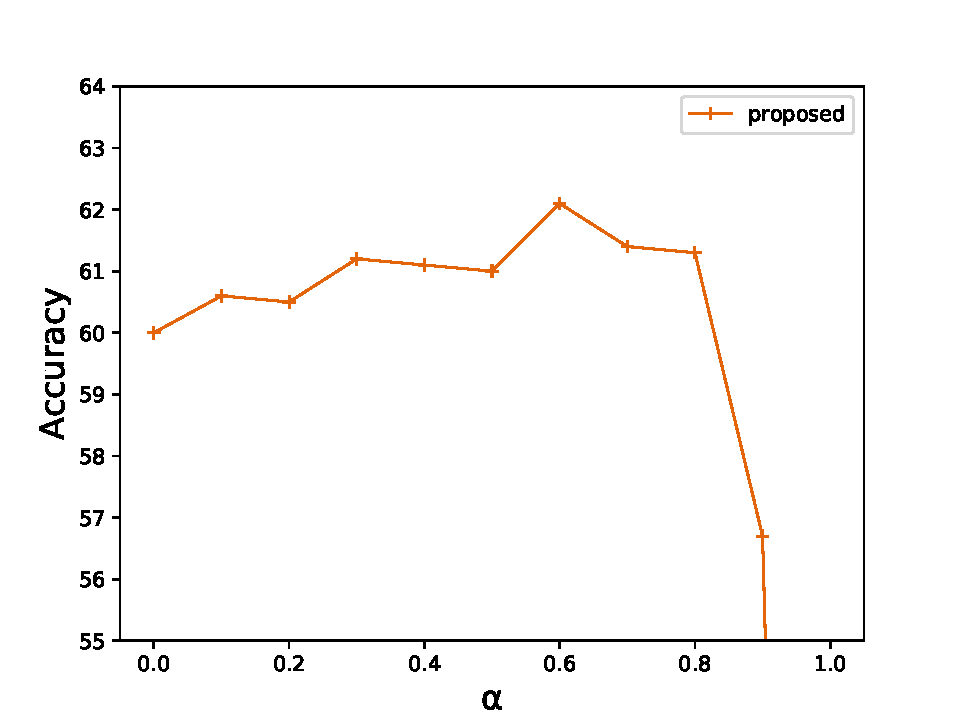
\includegraphics[width=12cm]{figures/citeseer_solo.pdf}
     \vspace*{0.5cm} 
    \caption{citeseerにおける比較} %タイトルをつける
    \label{citeseer_alpha} %ラベルをつけ図の参照を可能にする
\end{figure*}

\begin{figure*}[h]
  \centering
    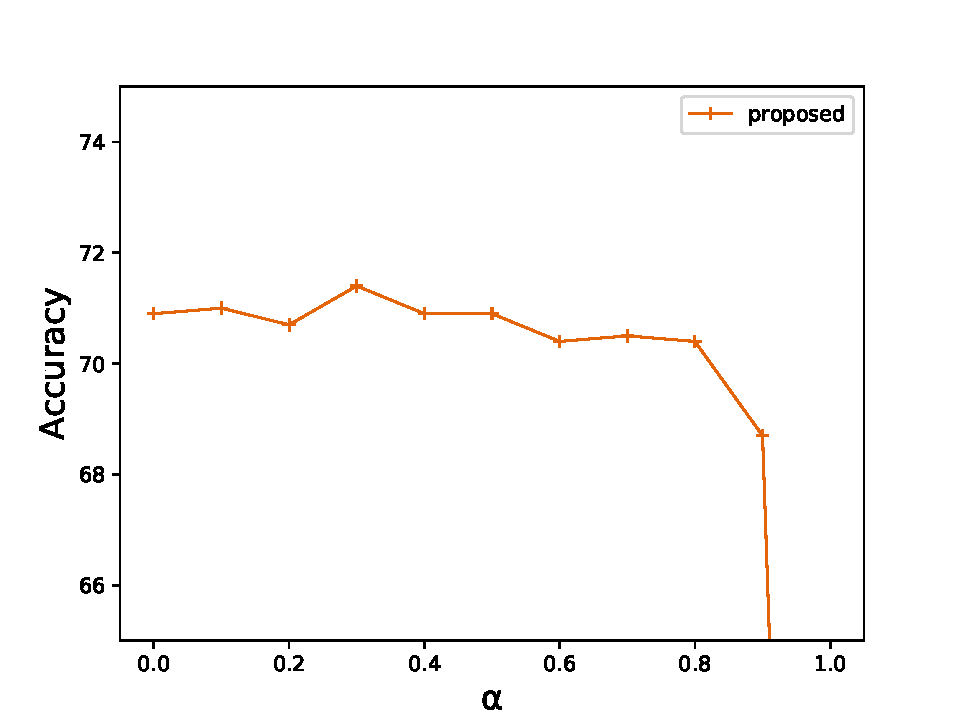
\includegraphics[width=12cm]{figures/pubmed_solo.pdf}
     \vspace*{0.5cm} 
    \caption{pubmedにおける比較} %タイトルをつける
    \label{pubmed_alpha} %ラベルをつけ図の参照を可能にする
\end{figure*}



%\chapter{Conclusion}
\chapter{結論}

結論はかくかくしかじか.結論はかくかくしかじか.

残された課題はかくかくしかじか.残された課題はかくかくしかじか.
残された課題はかくかくしかじか.残された課題はかくかくしかじか.

%\chapter*{Acknowledgements}
%\addchapter{Acknowledgements}
\chapter*{謝辞}
\addchapter{謝辞}

本研究にあたり、熱心にご指導いただきました指導教員の村田剛志准教授に深く
感謝いたします。また、いつも貴重な意見をいただいた村田研究室の皆様に深くお
礼申し上げます。

%\addchapter{References}
\addchapter{参考文献}

\bibliography{bunken} %hoge.bibから拡張子を外した名前
\bibliographystyle{junsrt} %参考文献出力スタイル

%\appendix
%\chapter{Proof of Theorem 1}\label{appendix1}
\chapter{定理1の証明}\label{appendix1}

%\chapter{Proof of Theorem 2}\label{appendix2}
\chapter{定理2の証明}\label{appendix2}

% ----------------------------------------------------------------------
\end{document}
